\documentclass[floatfix,aps,prd,amsmath,amssymb]{revtex4}

\usepackage{hyperref}
\usepackage{epsfig}
\usepackage{color}
\usepackage{graphicx}
\usepackage{float}
\usepackage{listing} %listings
\usepackage{braket}
\usepackage{mathtools}
\usepackage[noabbrev,capitalise]{cleveref} %for \cref in CKM-Mechanism.tex 
\providecommand{\e}[1]{\ensuremath{\times 10^{#1}}} %because my scientific notation wouldn't work: Kevin

\begin{document}
\title{The Lorentz Group and Singular Lorentz Transformations}
\author{Kevin Maguire (10318135)}
\date{\today}

\begin{abstract}
\textit{abstract}
\end{abstract}

\maketitle
\pagenumbering{roman}

%\begin{figure}[h!]
%\begin{center}
%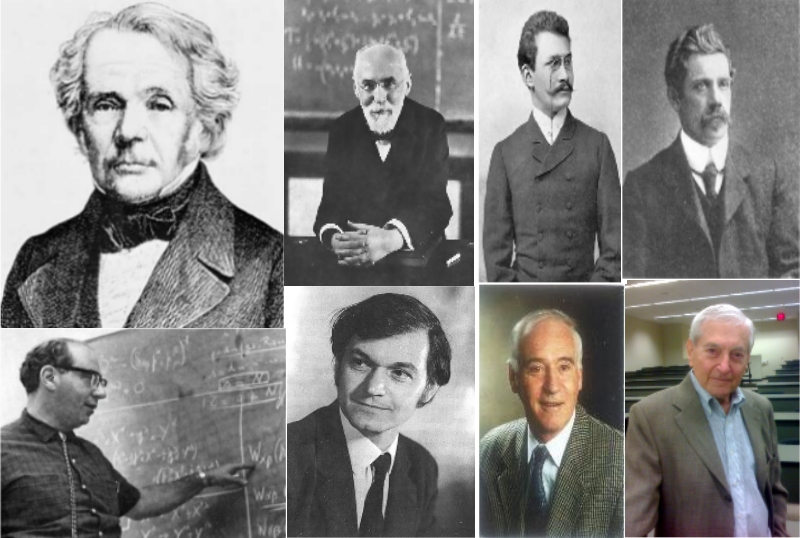
\includegraphics[scale=0.8]{figs/Cover.jpg}
%\end{center}
%\caption{\textit{}}
%\label{}
%\end{figure}

\newpage

\tableofcontents
\pagenumbering{arabic}

\newpage
 
\section{The Lorentz Transformation}

In this section the two null directions inherent in all Lorentz transformations, except the singular Lorentz transformations, are illustrated. The Lorentz Transform is defined by $(x,y,z,t) \rightarrow (x',y',z',t')$ such that

\begin{equation*}
{x'}^2 + {y'}^2 + {z'}^2 - {t'}^2 = x^2 + y^2 + z^2 - t^2.
\end{equation*}

\noindent If the transformation preserves the orientation of the spatial axes then is it called a \textit{proper} Lorentz transformation. This is equivalent to saying the transformation does not change the handedness of the axes. Also if $t \geq 0$ implies that time is always positive then it is called an \textit{orthochronous} Lorentz transformation, which ensures that the time direction is preserved. In this project the ``Lorentz transformation'' will refer to the proper, orthochronous Lorentz transformation.

Consider a photon moving in the $x$ direction at the speed of light, $c = 1$, and starting at $x = 0$. The space-time for such a photon can be illustrated as in Fig.() (FIGURE). It is clear that there are two null directions in this space-time, $x = \pm t$. To see this use the standard Lorentz transformation

\begin{align*}
x'  = \gamma (x - vt),  \\
t'  = \gamma (t - vx),
\end{align*}

\noindent where $\gamma = {(1 - v^2)}^{-1/2}$. Rearrange to obtain

\begin{eqnarray*}
x' - t' = \gamma (1 + v) (x - t), \\
x' + t' = \gamma (1 - v) (x + t).
\end{eqnarray*}

\noindent It is clear that $x = \pm t$ implies $x' = \pm t'$. Thus there are two null directions in this space-time at $x = \pm t$, as null directions are by definition invariant under a Lorentz transformation. It can be shown that all Lorentz transformations have two invariant null directions except the singular Lorentz transformation which has only one fixed null direction.  


\section{Reparameterisation of the Schwarzschild Solution}

In this section the Kasner solution of the vacuum field equations is derived from the Schwarzschild solution by taking the limit as the mass goes to infinity. It is then shown that the special case of the Kasner solution with no mass is equivalent to a novel form of Minkowskian space-time. Start with the Schwarzschild Solution of the vacuum field equations given by

\begin{equation}\label{Schwarz_Sol} 
\epsilon {\mathrm{d}s}^2 = {\left(1 - \frac{2m}{r}\right)}^{-1} {\mathrm{d}r}^{2} + r^2 ({\mathrm{d}\theta}^2 + {{\sin}^2 \theta}{\mathrm{d} \phi}^2) - \left(1 - \frac{2m}{r}\right) {\mathrm{d}t}^2.
\end{equation}

\subsection{Eddington-Finkelstein Coordinate Transformation}\label{Ed_Finkel_section}

\noindent First, make the Eddington-Finkelstein coordinate transformation

\begin{equation}\label{Ed-Fin_trans}
u = t - r - 2m \ln(r - 2m).
\end{equation}

\noindent This is generally used for a Schwarzschild geometry, particularly black holes. It is useful as it removes the singularity at the origin \cite{Finkelstein_Paper}. Calculate the differentials

\begin{align*}
\mathrm{d}u & = \mathrm{d}t - \mathrm{d}r - \frac{2m \mathrm{d}r}{r - 2m},\\
            & = \mathrm{d}t - \mathrm{d}r{\left( 1-\frac{2m}{r}  \right)}^{-1},\\
\mathrm{d}t & = \mathrm{d}u + {\left( 1-\frac{2m}{r}  \right)}^{-1} \mathrm{d}r, 
\end{align*}

\noindent and sub them into Eqn.(\ref{Schwarz_Sol}).

\begin{equation*}
\epsilon {\mathrm{d}s}^{2} = {\left( 1-\frac{2m}{r}  \right)}^{-1} \mathrm{d}r^2 + r^2 ({\mathrm{d}\theta}^2 + {{\sin}^2 \theta}{\mathrm{d} \phi}^2) - {\left( 1-\frac{2m}{r}  \right)} {\left( \mathrm{d}u + {\left( 1-\frac{2m}{r}  \right)}^{-1} \mathrm{d}r \right)}^{2},
\end{equation*}

\noindent which gives the result,

\begin{equation}\label{Reparameterisation_Schwarzschild_Before_Limit}
\epsilon {\mathrm{d}s}^{2} = r^2 ({\mathrm{d}\theta}^2 + {{\sin}^2 \theta}{\mathrm{d} \phi}^2) - 2 \mathrm{d}u \mathrm{d}r - {\mathrm{d}u}^{2} + \frac{2m}{r} {\mathrm{d}u}^{2}. 
\end{equation}

Note that if $m = 0$ the space-time becomes Minkowskian, as expected. If $r = 0$ in this Minkowskian space-time the line element becomes

$$ \epsilon {\mathrm{d}s}^2 = - {\mathrm{d}u}^{2},$$

\noindent which implies that $\epsilon = -1$ and the first integral of this trajectory is also equal to $-1$. Thus $r = 0$ is a time-like world-line in Minkowskian space-time, with proper time u. It can also be shown that $r=0$ is a geodesic with proper time, $u$ an affine parameter along it, this is done here in two ways. The first method is to write the line element in Cartesian coordinates using the transformation

\begin{gather*} 
x = r\sin{\theta}\cos{\phi}, \\
y = r\sin{\theta}\sin{\phi}, \\
z = r\cos{\theta}, \\
t = u + r.
\end{gather*}

\noindent It is clear that setting $r=0$ will give $x = y = z = 0$ and $t = u$. So the world-line is the t-axis with $u$ a parameter along it and is of course a time-like geodesic. The second method is much longer and involves calculating the metric and proving the geodesic equations, it is done here as it will be familiar to many readers. The Lagrangian method described by the following equations is used

\begin{gather*}
L = g_{ij} \dot{x}^{i}\dot{x}^{j},\\
\frac{d}{ds}\left( \frac{\partial L}{\partial \dot{x}^{i}}\right) - \frac{\partial L}{\partial {x}^{i}} = 2 w_{i}, \\
w^{j} = g^{ji}w_{i},  
\end{gather*}

\noindent with a geodesic defined by $w^{j} = 0$. The metric of this space-time in coordinates $(r ,\theta, \phi, u)$ is determined from Eqn.(\ref{Reparameterisation_Schwarzschild_Before_Limit}) with $m=0$

\begin{equation*}
g_{ij} = 
\left(
\begin{array}{cccc}
0  & 0 & 0             & -1 \\
0  & r & 0             & 0  \\
0  & 0 & r\sin{\theta} & 0  \\
-1 & 0 & 0             & -1 \\
\end{array}
\right).
\end{equation*}

\noindent The inverse of the metric is calculated to be

\begin{equation*}
g^{ij} =
\left(
\begin{array}{cccc}
1  & 0           & 0                       & -1 \\
0  & \frac{1}{r} & 0                       & 0  \\
0  & 0           & \frac{1}{r\sin{\theta}} & 0  \\
-1 & 0           & 0                       & 0  \\
\end{array}
\right).
\end{equation*}

\noindent $w^{j}$ will be calculated for $r$ and $u$ and simply stated for $\theta$ and $\phi$. The Lagrangian for $r$ is

\begin{equation*}
w_{r} = - \ddot{u} - r (\dot{\theta}^2 + \sin^2{\theta}\dot{\phi}^2),
\end{equation*}

\noindent and the Lagrangian for $u$ is

\begin{equation*}
w_{u} = - \ddot{u} - \ddot{r}  
\end{equation*}
 
\noindent Now $w^{r}$ is given by

\begin{align*}
w^{r} & = g^{rj} w_{j} \\
      & = w_{r} - w_{u}
\end{align*}

\noindent and $w^{u}$ is

\begin{align*}
w^{u} & = g^{uj} w_{j} \\
      & =  - w_{r}
\end{align*}

\noindent So putting these together to obtain $w^{r} = 2w_{r}$ and $w^{u} = -w_{r}$ which implies

\begin{align*}
w^{r} & = -2 \ddot{u} - 2 r(\dot{\theta}^2 + \sin^2{\theta}\dot{\phi}^2), \\
w^{u} & = \ddot{u} + r(\dot{\theta}^2 + \sin^2{\theta}\dot{\phi}^2), \\
\end{align*}

\noindent and also for $\theta$ and $\phi$

\begin{align*}
w^{\theta} = r \ddot{\theta} + 2 \dot{\theta} \dot{r} - r \sin{\theta}\cos{\theta}\dot{\phi}^2, \\
w^{\phi} = \sin{\theta}(\dot{\phi} \dot{r} + r \ddot{\phi}) + 2r \dot{\phi}\cos{\theta} \dot{\theta}.
\end{align*}

\noindent Then set $r=0$ to obtain the equations

\begin{align*} 
w^{r} = - 2 \ddot{u}, \\
w^{u} = \ddot{u}, \\
w^{\theta} = 0, \\
w^{\phi} = 0,.
\end{align*} 

\noindent Now $s = u$ as $u$ is proper time then $w^{r} = w^{u} = 0$, which implies that the trajectory $r=0$ is a geodesic with $u$ an affine parameter along it. 

The limit of the Schwarzschild solution as $m \rightarrow \infty$ must be calculated to find the Kasner solution. In its current form the limit cannot be taken, so two suitable coordinate transformations must be made to get it in a more useful form. First Set 

\begin{gather*} 
u = \mu u', \\
r = {\mu}^{-1} r',   
\end{gather*} 

\noindent where $\mu = \text{ const}$ so that
  
\begin{gather*} 
\mathrm{d}u = \mu \mathrm{d}u', \\
\mathrm{d}r = {\mu}^{-1} \mathrm{d}r'. \\
\end{gather*} 

\noindent The product of the differentials is then invariant

\begin{equation*}
{\mathrm{d}u}{\mathrm{d}r} = {\mathrm{d}u'}{\mathrm{d}r'}. 
\end{equation*}

\noindent When the new coordinates are subbed into Eqn.(\ref{Reparameterisation_Schwarzschild_Before_Limit}) the Schwarzschild solution becomes

\begin{equation}\label{Reparameterise_Schwarzschild_Next_Before_Limit}
\epsilon {\mathrm{d}s}^2 = {r'}^2 \sin^2 \theta \left\{ \frac{{\mathrm{d}\theta}^2}{\mu^2 \sin^2 \theta} +  \mu^{-2} {\mathrm{d} \phi}^2 \right\} - 2 {\mathrm{d}u'} {\mathrm{d}r'} - \left( \mu^2 - \frac{2 m \mu^3}{r'}\right) {\mathrm{d}u'}^2 . 
\end{equation}

\noindent Now set $m \mu^{3} = k$ or $ m = k \mu^{-3}$ and make another transformation first done by Ivor Robinson given by \cite{I_Robinson_Paper}

\begin{align*} 
\sin{\theta} = \frac{1}{\cosh{(\mu \xi)}}, \qquad  \mu^{-1} \phi = \eta.  
\end{align*} 

\noindent The second of these transformations gives simply $\mu^{-2} \mathrm{d}\phi^2 = \mathrm{d} \eta^2$. To rewrite the first coordinate transformation, first differentiate.

\begin{align*} 
\cos{\theta} \mathrm{d} \theta & = \frac{-1}{(\cosh(\mu \xi))^{2}} \sinh(\mu \xi) \mu \mathrm{d} \xi, \\
                      & = -{\sin}^{2}\theta \sinh(\mu \xi) \mu \mathrm{d} \xi.
\end{align*}

\noindent Use the formula $\cosh^2 A - \sinh^2 A = 1$, divide by $\mathrm{d} \xi$ and simplify using trigonometric identities

\begin{align*}
\cos{\theta} \frac{\mathrm{d} \theta}{\mathrm{d} \xi} & = -\mu \sin^2 \theta \sqrt{\frac{1}{\sin^2 \theta} - 1}, \\
                                    & = - \mu \sin \theta \cos \theta.
\end{align*}

\noindent Finally rewrite in terms of $\mathrm{d} \xi$

\begin{equation*}
\mathrm{d} \xi^2 = {\left( \frac{\mathrm{d} \theta}{\mu \sin \theta}  \right)}^2.
\end{equation*}

\noindent Subbing these transformations into Eqn.(\ref{Reparameterise_Schwarzschild_Next_Before_Limit}) gives

\begin{equation*}
\epsilon {\mathrm{d}s}^2 = \frac{r^2}{\cosh^{2}{\mu \xi}} ({\mathrm{d}\xi}^2 + {\mathrm{d}\eta}^2) - 2 {\mathrm{d}u}{\mathrm{d}r} - \left( \mu^{2} - \frac{2k}{r} \right) {\mathrm{d}u}^2,
\end{equation*}

\noindent where the primes have been dropped for convenience. 

\subsection{The Kasner Solution}

This is now in an appropriate form to take the limit $m \rightarrow \infty$ which is equivalent to $\mu \rightarrow 0$, to obtain

\begin{equation}\label{Kasner_after_limit}
\epsilon {\mathrm{d}s}^2 = r^2 ({\mathrm{d}\xi}^2 + {\mathrm{d}\eta}^2) - 2 {\mathrm{d}u}{\mathrm{d}r} - \frac{2k}{r} {\mathrm{d}u}^2
\end{equation}

\noindent This is still a solution of the field equations but it is no longer the Schwarzschild solution. In this section it is shown to be the Kasner Solution, which by definition is given by

\begin{equation}\label{Reparameterise_Definition_Of_Kasner} 
\epsilon {\mathrm{d}s}^2 = T^{2p} {\mathrm{d}X}^2 + T^{2q} \mathrm{d}Y^2 + T^{2r} \mathrm{d}Z^2 - \mathrm{d}T^2,
\end{equation}

\noindent such that

\begin{eqnarray*}
p + q + r = 1 = p^2 + q^2 + r^2.
\end{eqnarray*}

This solution is characteristic of aniosotropic space-times, which means it is directionally dependant. To write Eqn.(\ref{Kasner_after_limit}) in the above form first make the transformation

\begin{gather*} 
\xi' = \lambda^{-1} \xi, \text{    }  \eta' = \lambda^{-1} \eta, \\
r' = \lambda r,          \text{    }  u' = \lambda^{-1} u,
\end{gather*}

\noindent with $\lambda \vcentcolon = k^{-1/3}$. Subbing in these new coordinates gives

\begin{equation*}  
\epsilon \mathrm{d} s^2 = {r'}^2 (\mathrm{d} {\xi'}^2 + \mathrm{d} {\eta'}^2) - 2 \mathrm{d} u' \mathrm{d} r' + \frac{2}{r'}\mathrm{d} {u'}^2.
\end{equation*}

\noindent Now add and subtract $(r'/2) \mathrm{d} {r'}^2$ to complete the square as follows

\begin{equation*}  
\epsilon \mathrm{d} s^2 = r^2 (\mathrm{d} \xi^2 + \mathrm{d} \eta^2) + \frac{2}{r}{\left( \mathrm{d} u  - \frac{r}{2} \mathrm{d} r\right)}^2 - \frac{r}{2}\mathrm{d} r^2,
\end{equation*}

\noindent where the primes have again been dropped for convenience. Now set

\begin{equation*}
\bar{X} = u - \frac{r^2}{4},
\end{equation*}

\noindent so the differential of $\bar{X}$ is

\begin{equation*}
\mathrm{d} \bar{X} = \mathrm{d} u - \frac{r}{2} \mathrm{d}r,
\end{equation*}

\noindent and the line element can be rewritten in terms of $\bar{X}$,

\begin{equation*}
\epsilon \mathrm{d} s^2 = r^2 (\mathrm{d} \xi^2 + \mathrm{d} \eta^2) + \frac{2}{r} \mathrm{d} \bar{X}^2 - {\left( \frac{r^{1/2}}{\sqrt{2}} \mathrm{d} r\right)}^{2}.
\end{equation*}

\noindent Now define $T$ such that

\begin{equation*}
T = \frac{\sqrt{2}}{3} r^{3/2} \text{,       and    } r = {\left( \frac{3}{\sqrt{2}} \right)}^{2/3} T^{2/3},
\end{equation*}

\noindent which results in the new line element

\begin{equation*}
\epsilon \mathrm{d} s^2 = \left( \frac{3}{\sqrt{2}} \right)^{4/3} T^{4/3} (\mathrm{d} \xi^2 + \mathrm{d} \eta^2) + 2 \left( \frac{\sqrt{2}}{3}\right)^{2/3} T^{-2/3} \mathrm{d} \bar{X}^2 - \mathrm{d} T^2.
\end{equation*}

\noindent Then a final coordinate transformation can be made to remove the unwanted constants, given by

\begin{align*} 
X & = \left[ 2\left( \frac{\sqrt{2}}{3}\right)\right]^{1/2} \bar{X}, \\
Y & = \left( \frac{3}{\sqrt{2}} \right)^{2/3} \xi, \\
Z & = \left( \frac{3}{\sqrt{2}} \right)^{2/3} \eta, \\
\end{align*} 

\noindent to obtain

\begin{equation}\label{Our_Kasner} 
\epsilon {\mathrm{d}s}^2 = T^{-2/3} {\mathrm{d}X}^2 + T^{4/3} \left( \mathrm{d}Y^2 + \mathrm{d}Z^2 \right) - \mathrm{d}T^2.
\end{equation}

\noindent Comparing this result to the general form of the Kasner solution in Eqn.(\ref{Reparameterise_Definition_Of_Kasner}) it is clear that they have the same form with $p=-1/3$ and $q=r=2/3$. Thus the solution obtained by taking the limit of the Schwarzschild solution as $m \rightarrow \infty$ is indeed the Kasner Solution. 

\subsection{Line Element of Minkowskian Space-Time}

Minkowskian space-time reemerges again by setting the energy, $k = 0$ in Eqn.(\ref{Kasner_after_limit}), which is equivalent to $m = 0$. 

\begin{equation}\label{Kasner_after_limit_no_k}
\epsilon {\mathrm{d}s}^2 = r^2 ({\mathrm{d}\xi}^2 + {\mathrm{d}\eta}^2) - 2 {\mathrm{d}u}{\mathrm{d}r}
\end{equation}

\noindent Setting $r = 0$ gives $\epsilon {\mathrm{d}s}^2 = 0$. In this section it is demonstrated that $r = 0$ is a null geodesic with $u$ an affine parameter along it and that Eqn.(\ref{Kasner_after_limit_no_k}) is indeed the Minkowskian space-time line element. To verify these properties first let $x^i = (x,y,z,t)$ be rectangular Cartesian coordinates with time in Minkowskian space-time with the usual line element

\begin{equation*} 
\epsilon {\mathrm{d}s_0}^2 = {\mathrm{d}x}^2 + {\mathrm{d}y}^2 + {\mathrm{d}z}^2 - {\mathrm{d}t}^2.
\end{equation*} 

\noindent We note that the trajectory $C$  defined by $x = 0$, $y = 0$, $z = t$ is a null geodesic as it will lie on the light cone of Minkowskian space-time. 

\begin{figure}[h!]
\begin{center}
\caption{\textit{Minkowskian space-time illustrating the new parameter $r$ which is the shortest distance between some point $x^i$ and the trajectory $C$ along the $k^i$ direction. The parameter $u$ which determines the distance travelled along $C$ is also shown}}
\label{Reparameterization_Figure_Unit_Vector}
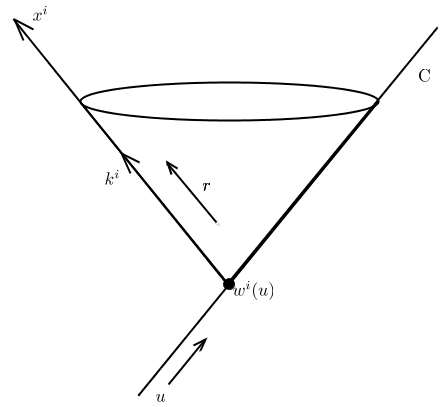
\includegraphics[scale=0.8]{figs/2_1.png}
\end{center}
\end{figure}

\noindent If $C$ is written parametrically as $x^i = w^i (u)$ such that $w^i = (0,0,u,u)$ then $u$ is an affine parameter along it. The tangent to $C$ is then computed as

\begin{equation*} 
v^i (u) = \frac{\mathrm{d} w^i}{\mathrm{d}u} = (0,0,1,1).
\end{equation*} 

\noindent As $C$ is a null geodesic the first integral will be $v_i v^i = 0$ and thus $v_i = (0,0,1,-1)$ where we have chosen the convention $(+,+,+,-)$. The position vector of a point in Minkowskian space time can be written in the form

\begin{eqnarray*}
x^i - w^i (u) = r k^i, \\
\text{or } x^i = w^i(u) + r k^i. 
\end{eqnarray*}

\noindent Thus $r$ is a new parameter which gives the shortest distance between $C$ and some point $x^i$, and $k^i$ is the unit vector in that direction, see Fig.(\ref{Reparameterization_Figure_Unit_Vector}). As $k^i$ is a unit vector it satisfies the relations

\begin{gather}
k^i k_i = 0 \label{k_rel_1},\\
k^i v_i = -1 \label{k_rel_2}.
\end{gather}

\noindent Thus $k^i$ is normalized so that $k^i$ and $v^i$ are both future pointing. Making the parameterisation

\begin{gather*}
k^i = (\xi, \eta, A, B), \\
k_i = (\xi, \eta, A, -B).
\end{gather*}

\noindent We can choose any variable for the first two slots of $k^i$ so we choose $\xi$ and $\eta$ from before for convenience. Using the relation (\ref{k_rel_1}) it is clear that

\begin{equation*}
\xi^2 + \eta^2 + A^2 - B^2 = 0,
\end{equation*}

\noindent and using the relation (\ref{k_rel_2}) it is found that

\begin{gather}
A - B = -1 \label{sim_rel_1},\\
A^2 - B^2 = (A + B)(A - B) = - (A + B).
\end{gather}

\noindent Which implies

\begin{equation}\label{sim_rel_2}
\xi^2 + \eta^2 = A + B. 
\end{equation}

\noindent So expressions for $A$ and $B$ are found using Eqn.(\ref{sim_rel_1}) and Eqn.(\ref{sim_rel_2}):

\begin{eqnarray*}
A = \frac{1}{2} (-1 + \xi^2 + \eta^2) \\
B = \frac{1}{2} (1 + \xi^2 + \eta^2) \\
\end{eqnarray*}

In summary so far we have

\begin{align}
x^i & = w^i (u) + r k^i \label{rel_for_trans_1},\\
w^i & = (0,0, u,u) \label{rel_for_trans_2},\\
k^i & = (\xi, \eta, \frac{1}{2} (-1 + \xi^2 + \eta^2), \frac{1}{2} (1 + \xi^2 + \eta^2)) \label{rel_for_trans_3},\\
x^i & = (x, y, z, t) \label{rel_for_trans_4}.  
\end{align}

Consider Eqn.(\ref{rel_for_trans_1}) as a coordinate transformation from $(x,y,z,t)$ to $(\xi,\eta, r, u )$ such that

\begin{align}
x & = r \xi, \nonumber \\
y & = r \eta, \nonumber \\
z & = u + \frac{r}{2} (-1 + \xi^2 + \eta^2), \nonumber \\
t & = u + \frac{r}{2} (1 + \xi^2 + \eta^2),  \label{trans_x_to_xi} 
\end{align} 

\noindent which is clear from Eqns.(\ref{rel_for_trans_1}) - (\ref{rel_for_trans_4}). Now this is applied to the Minkowskian line element of Eqn.(\ref{Kasner_after_limit_no_k}). First, the $x$ and $y$ differentials are

\begin{eqnarray*} 
dx = r \mathrm{d}\xi + \xi \mathrm{d}r, \\
\mathrm{d}y = r \mathrm{d}\eta + \eta \mathrm{d}r. 
\end{eqnarray*} 

\noindent Which gives

\begin{equation}\label{differentials_1}
{\mathrm{d}x}^2 + {\mathrm{d}y}^2 = r^2 ({\mathrm{d}\xi}^2 + {\mathrm{d}\eta}^2) + 2 r \xi {\mathrm{d}\xi} {\mathrm{d}r} + 2 r \eta {\mathrm{d}\eta}{\mathrm{d}r} + (\xi^2 + \eta^2) {\mathrm{d}r}^2.
\end{equation}

\noindent Next, the $z$ and $t$ differentials

\begin{align*}
z + t & = 2 u + r (\xi^2 + \eta^2), \\
z - t & = - r, \\
{\mathrm{d}z} + {\mathrm{d}t} & = 2 \mathrm{d}u + (\xi^2 + \eta^2) \mathrm{d}r + 2 r \xi {\mathrm{d}\xi} + 2 r \eta {\mathrm{d}\eta}, \\
{\mathrm{d}z} - {\mathrm{d}t} & = - \mathrm{d}r. 
\end{align*}

\noindent Then using difference of two squares to obtain

\begin{equation}\label{differentials_2}
{\mathrm{d}z}^2 - {\mathrm{d}t}^2 = -2 {\mathrm{d}u}{\mathrm{d}r} - (\xi^2 + \eta^2) {\mathrm{d}r}^2 - 2 r \xi {\mathrm{d}\xi}{\mathrm{d}r} - 2 r \eta {\mathrm{d}\eta}{\mathrm{d}r}.
\end{equation}

\noindent Combining Eqn.(\ref{differentials_1}) and (\ref{differentials_2}) to get:

\begin{equation*}
{\mathrm{d}x}^2 + {\mathrm{d}y}^2 + {\mathrm{d}z}^2 - {\mathrm{d}t}^2 = r^2 ({\mathrm{d}\xi}^2 + {\mathrm{d}\eta}^2) - 2 {\mathrm{d}u}{\mathrm{d}r}
\end{equation*}

\noindent and from this it is clear that Eqn.(\ref{Kasner_after_limit_no_k}) is the line element of Minkowskian space-time with $r = 0$ a null geodesic with affine parameter $u$ along it as stated in Section (\ref{Ed_Finkel_section}).

Thus it has been shown that the Kasner solution to the vacuum filed equations can be obtained from the Schwarzschild solution of the vacuum field equations by taking the special case where the mass goes to infinity. Then the Minkowskian space-time line element in a particular set of coordinates $(\xi, \eta, r, u)$, can be derived from the Kasner solution by setting the energy, $k$ to zero. It has been shown that the special case where $r=0$ in this Minkowskian space-time is then a null geodesic with $u$ an affine parameter along it.  


\newpage

\begin{appendix}

\section{Singular Lorentz Transformation with Special Significance Given to $x$}\label{Appendix_Special_Significance_x}

The choice of components of the matrix $A$ in Eqn.(\ref{Special_Matrices_A_first}) gives an arbitrary but special significance to the corrdinate $z$. In this calculation the matrix $U$ of Eqn.(\ref{SL_trans}) is determined for a singular Lorentz transformation, in which special significance has been given to the coordinate $x$. This transformation is given by

\begin{align*}
t'-x' & = t-x, \\
z'+iy' & = z + iy + w(t-x), \\
t'+x' & = t+x + w(z-iy) + \bar{w} (z + iy) + w \bar{w} (t-x).
\end{align*}

\noindent Notice that this is the same tranformation as in Example 3, Section (\ref{Special_Linear_Matrices_Example_3}), with $x$ and $z$ swapped. This is equivalent to swapping these two coordinates in the matrix $A$ only. Note that if $x$ and $z$ were exchanged in both $A$ and the transformation then the $U$ obtained would be exactly the same as the example done previously.

First, the components of the matrix $A$ must be construced. Thus the transformation must be written out explicitly as 

\begin{align*}
x' & = x + \frac{1}{2} (w + \bar{w})z + \frac{i}{2}(\bar{w}- w)y + \frac{1}{2}w\bar{w}(t-x), \\
y' & = y + \frac{i}{2} (\bar{w} - w)(t-x), \\
z' & = z + \frac{1}{2} (w + \bar{w})(t-x), \\
t' & = t + \frac{1}{2} (w + \bar{w})z + \frac{i}{2} (\bar{w}-w)y + \frac{1}{2} w\bar{w}(t-x).
\end{align*}

\noindent Now construct the components of $A$

\begin{align*}
t' - z' & = t - z + \frac{1}{2}(w + \bar{w})z + \frac{i}{2} (\bar{w}-w)y + \frac{1}{2}w\bar{w}(t-x) - \frac{1}{2}(\bar{w} + w)(t-x),\\
t' + z' & = t + z + \frac{1}{2}(w + \bar{w})z + \frac{i}{2} (\bar{w}-w)y + \frac{1}{2}w\bar{w}(t-x) + -\frac{1}{2}(\bar{w} + w)(t-x),\\
x' + iy' & = x +  \frac{1}{2}(w + \bar{w})z + \frac{i}{2} (\bar{w}-w)y + \frac{1}{2}w\bar{w}(t-x) - \frac{1}{2}(\bar{w} + w)(t-x) + iy.
\end{align*}

\noindent Equating coefficients of $x$, $y$, $z$, $t$ on both sides of Eqn.(\ref{general_coeff_equate_a}) to obtain

\begin{subequations}
\begin{gather}\label{Ex_Ap_equate_coeffs_first_a}
\alpha \bar{\beta} + \bar{\alpha} \beta = \frac{1}{2}(\bar{w}+w) - \frac{1}{2}w\bar{w}, \\\label{Ex_Ap_equate_coeffs_first_b}
\alpha \bar{\beta} - \bar{\alpha} \beta = \frac{1}{2} (\bar{w} - w), \\\label{Ex_Ap_equate_coeffs_first_c}
-\alpha \bar{\alpha} + \beta \bar{\beta} = - 1 + \frac{1}{2}(\bar{w} + w), \\\label{Ex_Ap_equate_coeffs_first_d}
\alpha \bar{\alpha} + \beta \bar{\beta} = 1 + \frac{1}{2}w\bar{w} - \frac{1}{2}(\bar{w} + w). 
\end{gather}
\end{subequations}

\noindent Then Eqn.(\ref{Ex_Ap_equate_coeffs_first_a}) and (\ref{Ex_Ap_equate_coeffs_first_b}) imply $\alpha \bar{\beta} = \frac{1}{2}\bar{w} - \frac{1}{4}w\bar{w}$. Also Eqn.(\ref{Ex_Ap_equate_coeffs_first_c}) and (\ref{Ex_Ap_equate_coeffs_first_d}) imply $\beta\bar{\beta} = \frac{1}{4}w\bar{w}$ and $\alpha \bar{\alpha} = 1 + \frac{1}{4}w\bar{w} - \frac{1}{2}\bar{w} - \frac{1}{2}w$. Hence $\alpha$ can be written in terms of $\beta$

\begin{gather*}
\alpha \bar{\beta} = (\frac{1}{2}\bar{w} - \frac{1}{4}w\bar{w}), \\
\frac{1}{4} w \bar{w} \alpha = \frac{1}{2}\bar{w}(1-\frac{1}{2}w)\beta, \\
\alpha = \frac{(2-w)}{w}\beta.
\end{gather*}

Equating coefficients of $x$, $y$, $z$, $t$ on both sides of Eqn.(\ref{general_coeff_equate_b}) to obtain

\begin{subequations}
\begin{gather}\label{Ex_Ap_equate_coeffs_second_a}
\alpha \bar{\delta} + \beta\bar{\gamma} = 1 - \frac{1}{2}w\bar{w} + \frac{1}{2}(\bar{w}-w), \\\label{Ex_Ap_equate_coeffs_second_b}
\alpha \bar{\delta} - \beta\bar{\gamma} = \frac{1}{2}(\bar{w}-w) + 1,\\\label{Ex_Ap_equate_coeffs_second_c}
-\alpha\bar{\gamma} + \beta \bar{\delta} = \frac{1}{2}(\bar{w} + w) ,\\\label{Ex_Ap_equate_coeffs_second_d}
\alpha\bar{\gamma} + \beta \bar{\delta} = \frac{1}{2}w\bar{w} - \frac{1}{2}(\bar{w}-w). 
\end{gather}
\end{subequations}

\noindent Now Eqn.(\ref{Ex_Ap_equate_coeffs_second_a}) and (\ref{Ex_Ap_equate_coeffs_second_b}) imply $\beta \bar{\gamma} = -\frac{1}{4}w\bar{w}$. So using $\bar{\beta} \beta= \frac{1}{4}w\bar{w}$ again to obtain

\begin{gather*}
\frac{1}{4}w\bar{w} \bar{\gamma} = \bar{\beta}\beta\bar{\gamma},\\
\frac{1}{4}w\bar{w} \bar{\gamma} = -\frac{1}{4}w\bar{w} \bar{\beta},\\
\gamma = -\beta.
\end{gather*}

\noindent Also Eqn.(\ref{Ex_Ap_equate_coeffs_second_c}) and (\ref{Ex_Ap_equate_coeffs_second_d}) imply $\beta \bar{\delta} = \frac{1}{4}w\bar{w} + \frac{1}{2}w$. Thus

\begin{gather*}
\frac{1}{4}w\bar{w}\bar{\delta} = \left(\frac{1}{4}w\bar{w}+ \frac{1}{2}w\right)\bar{\beta},\\
\delta = \left(\frac{w\bar{w} + 2\bar{w}}{w\bar{w}}\right)\beta.
\end{gather*}

\noindent Equating coefficients of $x$, $y$, $z$, $t$ on both sides of Eqn.(\ref{general_coeff_equate_c}) to obtain

\begin{subequations}
\begin{gather}\label{Ex_Ap_equate_coeffs_third_a}
\gamma \bar{\delta} + \delta \bar{\gamma} = -\frac{1}{2}w\bar{w} - \frac{1}{2}(w + \bar{w}), \\\label{Ex_Ap_equate_coeffs_third_b}
\gamma \bar{\delta} - \delta \bar{\gamma} =  \frac{1}{2}(\bar{w}-w),\\\label{Ex_Ap_equate_coeffs_third_c}
-\gamma \bar{\gamma} + \delta \bar{\delta} = 1 + \frac{1}{2}(w + \bar{w}),\\\label{Ex_Ap_equate_coeffs_third_d}
\gamma \bar{\gamma} + \delta \bar{\delta} = 1 + \frac{1}{2}w\bar{w} + \frac{1}{2}(\bar{w}+w). 
\end{gather}
\end{subequations}

\noindent Here Eqn(\ref{Ex_Ap_equate_coeffs_third_a}) and (\ref{Ex_Ap_equate_coeffs_third_b}) imply $\gamma \bar{\delta} = -\frac{w}{4}(2+\bar{w})$. Also, Eqn(\ref{Ex_Ap_equate_coeffs_third_c}) and Eqn(\ref{Ex_Ap_equate_coeffs_third_d}) imply $\gamma \bar{\gamma} = \frac{1}{4}w\bar{w}$. So using these relations $\delta$ can be written in terms of $\gamma$ 

\begin{gather*}
\gamma \bar{\gamma} \bar{\delta} = \frac{w}{4}(2+\bar{w})\bar{\gamma},\\
\frac{1}{4}w\bar{w} \bar{\delta} = \frac{w}{4}(2+\bar{w})\bar{\gamma},\\
\delta = -\frac{(2 + w)}{w}\gamma.
\end{gather*}

\noindent At this point $\beta$ and $\delta$ have been written in terms of $\gamma$ and $\alpha$ is written in terms of $\beta$. Write $\alpha$ in terms of $\gamma$

\begin{equation*}
\alpha = \frac{(2-w)}{w}\beta = \frac{(w-2)}{w}\gamma.
\end{equation*}

\noindent Now use the condition that $\det{(U)} = 1$ and replace everything in favour of $\gamma$

\begin{gather*}
\alpha \delta - \beta \gamma = 1,\\
-\frac{(w^2 - 4)}{w^2}\gamma^2 + \gamma^2 = 1,\\
\frac{4}{w^2}\gamma^2 = 1,\\
\gamma = \pm \frac{w}{2}.
\end{gather*}

\noindent Replace $\gamma$ and write all the components of $U$ as functions of $w$ only

\begin{align*}
\alpha & = \pm \frac{1}{2}(w-2),\\
\beta & = \mp \frac{w}{2},\\
\gamma & = \pm \frac{w}{2},\\
\delta & = \mp \frac{1}{2}(w+2).
\end{align*}

\noindent Finally it is found that 

\begin{equation*}
U = \pm
\left(
\begin{array}{ccc}
\frac{w-2}{2} & & -\frac{w}{2}     \\
 & & \\
\frac{w}{2}   & & -\frac{(w+2)}{2} \\
\end{array}
\right).
\end{equation*}

Now the fractional linear trasnformation associated with $U$ must be determined. Using Eqn.(\ref{Extended_Complex_Fractional_Linear_Transformation}) to find that

\begin{equation*}
\zeta' = \frac{\bar{w} - (\bar{w} +2)\zeta}{\bar{w} -2 - \bar{w}\zeta}. 
\end{equation*}

\noindent The fixed points of the system and thus the null directions are found by setting $\zeta' = \zeta$ to obtain

\begin{gather*}
\bar{w} \zeta^2 - 2 \bar{w} \zeta + \bar{w} = 0,\\
\bar{w}(\zeta-1)^2 = 0.
\end{gather*}

\noindent Thus there is a fixed point at $\zeta = 1$. The corresponding null direction is then given by Eqn.(\ref{Ext_Complex_vec_x_relations}) such that $\vec{x}= t(1,0,0,1)$. Hence finally the null direction is the generator of $N^+$, $x=t$. So in this case where $x$ was given special significance instead of $z$ with the given singular Lorentz transformation it is found that the null direction is $x=t$ instead of $z=t$. This is as expected as by exchanging $z$ with $x$ the coordinate system has been rotated. 

\section{Standard Lorentz Transformation of the Electromagnetic Field Vectors}\label{Appendix_Standard_Transform_EM_Vectors}

In this appendix the transformations laws for $\vec{E} = (E^1, E^2, E^3)$ and $\vec{B} = (B^1, B^2 B^3)$ under the standard Lorentz transformation of Eqn.(\ref{Special_Matrices_Standard_Lorentz}) are derived. If $p^i$ is any vector transported along $x^i = x^i (s)$ then, in Eqn.(\ref{Infinitesimal_DE_interms_v}), $v^i$ can be replaced with $p^i$, such that

\begin{equation*} 
\frac{\mathrm{d}p^i}{\mathrm{d}s} = \tensor{L}{^i_j} p^j.
\end{equation*} 

\noindent Here $s =$ arc length so the usual line element

\begin{equation*} 
\epsilon \mathrm{d}s^2 = \mathrm{d}x^2 + \mathrm{d}y^2 + \mathrm{d}z^2 - \mathrm{d}t^2,
\end{equation*} 

\noindent is formed. $p^i$ is a $4$-vector so it transforms like $x^i = (x,y,z,t)$ under the standard Lorentz transformation, such that

\begin{align*}
\bar{p}^1 = \gamma (p^1 - v p^4),\\
\bar{p}^2 = p^2, \\
\bar{p}^3 = p^3,\\
\bar{p}^4 = \gamma (p^4 - v p^1).
\end{align*}

\noindent Which implies that 

\begin{equation*}
\mathrm{d}p^i = (\mathrm{d}p^1,\mathrm{d}p^2,\mathrm{d}p^3,\mathrm{d}p^4),
\end{equation*}

\noindent is a $4$-vector and ds is invariant, thus $\frac{\mathrm{d}p^i}{\mathrm{d}s}$ is also a $4$-vector. Hence $\tensor{L}{^i_j} p^j$ is a $4$-vector for any $4$-vector $p^i$, where $\tensor{L}{^i_j}$ is given by

\begin{equation*}
\tensor{L}{^i_j} = 
\left(
\begin{array}
0    & B^3  & -B^2 & E^1 \\
-B^3 & 0    & B^1  & E^2 \\
B^2  & -B^1 & 0    & E^3 \\
E^1  & E^2  & E^3  & 0   \\
\end{array}
\right)
\end{equation*}

\noindent and a factor of $q/m$ has been left out as it will play no role. Write out $\tensor{L}{^i_j} p^j$ explicitly

\begin{align*}
\tensor{L}{^1_j}p^j & = B^3 p^2 - B^2 p^3 + E^1 p^4, \\
\tensor{L}{^2_j}p^j & = -B^3 p^1 + B^1 p^3 + E^2 p^4, \\
\tensor{L}{^3_j}p^j & = B^2 p^1 - B^1 p^2 + E^3 p^4, \\
\tensor{L}{^4_j}p^j & = E^1 p^1 + E^2p^2 + E^3 p^3.
\end{align*}

\noindent Since $\tensor{L}{^i_j} p^j$ is a $4$-vector it transforms under the standard Lorentz transformation, such that

\begin{align}
\label{Appendix_Lp_Standard_Transform_a}
\tensor{\bar{L}}{^1_j}\bar{p}^j = \gamma (\tensor{L}{^1_j}p^j - v \tensor{L}{^4_j}p^j),
\\\label{Appendix_Lp_Standard_Transform_b}
\tensor{\bar{L}}{^2_j}\bar{p}^j = \tensor{L}{^2_j}p^j,
\\\label{Appendix_Lp_Standard_Transform_c}
\tensor{\bar{L}}{^3_j}\bar{p}^j = \tensor{L}{^3_j}p^j,
\\\label{Appendix_Lp_Standard_Transform_d}
\tensor{\bar{L}}{^4_j}\bar{p}^j = \gamma(\tensor{L}{^4_j}p^j - v \tensor{L}{^1_j}p^j).
\end{align}

(ERROR. DONE TO HERE)


















\section{The Triad of Electromagnetic Radiation}\label{Appendix_Orthonormal_Triad}

In this appendix it is shown that the vectors $(\vec{n}, \vec{B}, \vec{E})$ form a right-handed triad. From Eqn.(\ref{Infinitesimal_K_Unit_Vector_Formula}), $k^i$ can be rewritten as

\begin{equation*}
k^i = (\zeta \bar{\zeta} + 1)(\vec{n}, 1),
\end{equation*}

\noindent where $\vec{n} = (n^1, n^2, n^3)$ is a unit vector such that $\vec{n} \cdot \vec{n} = 1$. Expanding the relation $\mathcal{L}_{ij} k^i = 0$ in terms of $\vec{n}$ gives

\begin{subequations}
\begin{align}
\label{Appendix_2_Expand_L_K_product_a}
(B^3 - i E^3)n^2 - (B^2 - i E^2)n^3 + E^1 + iB^1 & = 0, 
\\\label{Appendix_2_Expand_L_K_product_b}
-(B^3 - i E^3)n^1 + (B^1 - i E^1)n^3 + E^2 + iB^2 & = 0, 
\\\label{Appendix_2_Expand_L_K_product_c}
(B^2 - i E^2)n^1 - (B^1 - i E^1)n^2 + E^3 + iB^3 & = 0, 
\\\label{Appendix_2_Expand_L_K_product_d}
-(E^1 + i B^1)n^1 - (E^2 + iB^2)n^2 - (E^3 + iB^3) & = 0.
\end{align}
\end{subequations}

\noindent Then by equating real and imaginary parts of Eqn.(\ref{Appendix_2_Expand_L_K_product_d}) it is clear that  $\vec{E} \cdot \vec{n} = \vec{B} \cdot \vec{n}$. Also, from Eqns.(\ref{Appendix_2_Expand_L_K_product_a}) - (\ref{Appendix_2_Expand_L_K_product_c}) the following series of equations are seen, first Eqn.(\ref{Appendix_2_Expand_L_K_product_a}) implies

\begin{align*}
E^1 & = B^2 n^3 - B^3 n^2, \\
B^1 & = E^3 n^2 - E^2 n^3, 
\end{align*}

\noindent while Eqn.(\ref{Appendix_2_Expand_L_K_product_b}) gives

\begin{align*} 
E^2 & = B^3 n^1 - B^1n^3, \\
B^2 & = E^1 n^3 - E^3 n^1.
\end{align*} 

\noindent Then Eqn.(\ref{Appendix_2_Expand_L_K_product_c}) implies

\begin{align*}
E^3 & = B^1 n^2 - B^2 n^1,\\
B^3 & = E^2 n^1 - E^1 n^2.
\end{align*}

\noindent Thus is it clear that these are the components of the curl $\vec{E} = \vec{B} \times \vec{n}$ and $\vec{B} = \vec{n} \times \vec{E}$. This curl is proof that the vectors $(\vec{n}, \vec{E}, \vec{B})$ form a right-handed triad. 




\end{appendix}

 
\section{Acknowledgements}
 
\begin{thebibliography}{10}
%\bibitem{CPT}
%Hilary Greaves and Terugi Thomas - ``The CPT Theorem" - April 2012, \url{http://arxiv.org/abs/1204.4674}
\end{thebibliography}

\end{document}
